\documentclass[]{article}
\oddsidemargin=-5mm
\evensidemargin=-5mm\marginparwidth=.08in \marginparsep=.01in
\marginparpush=5pt\topmargin=-15mm\headheight=12pt
\headsep=25pt
\footskip=30pt
\textheight=25cm
\textwidth=17cm
\columnsep=2mm
\columnseprule=1pt\parindent=15pt\parskip=2pt
\usepackage[utf8]{inputenc}
\usepackage{graphicx}
\usepackage{amsmath} % Equations
    \usepackage{amssymb} % Equations

\begin{document}
\begin{center}
\bf Semestralní projekt MI-PDP 2018/2019:\\[5mm]
    Paralelni algoritmus pro řešení problému pokrývání plochy dlaždicemi L\\[5mm] 
       Ladislav Martínek\\[2mm]
magisterske studijum, FIT CVUT, Thakurova 9, 160 00 Praha 6\\[2mm]
\today
\end{center}

\section{Definice problému}

Problém, který jsme měli v ráncí semestrálního projektu řešit se týkal pokrývání plochy dlaždicemi L. Tedy bylo nutné pokrýt obdelníkovou mřížku dlaždicemi tak, že se optimalizovala cena takového řešení daná funkcí, která je uveden níže. 


\subsection{Vstupní data}
$m$, $n$ = rozměry obdélníkové mřížky $R[1..m,1..n]$, skládající se z $m$ x $n$ políček.
Dlaždice dvou tvarů L3 a L4, viz obrázek níže \ref{obr1}.

\begin{center}
 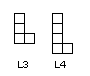
\includegraphics{ll.png}
 \label{obr1}
\end{center}

\noindent
$k <m*n $ = počet zakázaných políček v mřížce $R$.

\noindent
$D[1..k]$ = pole souřadnic $k$ zakázaných políček náhodně rozmístěných v mřížce $R$.

\noindent
Pro mřížku $R$ se zakázanými políčky danými polem $D$ najděte \textbf{pokrytí}  dlaždicemi L3 a L4 (viz obrázek \ref{obr1}) \textbf{s~maximální cenou}.
Dlaždice lze \textbf{pravoúhle otáčet} a \textbf{obracet} (viz obrázek \ref{obr2}).

\begin{center}
    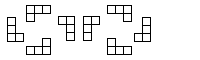
\includegraphics{l2.png}
     \label{obr2}
    \end{center}
  
 \noindent 
Všechna možná otočení a obrácení dlaždice L3.

\noindent
\textbf{Cena} pokrytí (funkce, kterou v algoritmu optimalizuji), ve kterém zbylo $q$ nepokrytých nezakázaných políček, je zadána následovně: 

$$ 2 * \text{počet dlaždic tvaru L3} + 3 * \text{počet dlaždic tvaru L4} - 6*q. $$

\subsection{Výstup algoritmu}

Číslo udávající maximální cenu pokrytí a počty dlaždic L3 a L4 a počet nepokrytých políček a jejich souřadnice.

\noindent
Popis pokrytí mřížky $R$, např. $(m \cdot n)$ - maticí identifikátorů, kde každá dlaždice je jednoznačně určena políčky 
s unikátním ID $>=1$, nepokrytá políčka jsou prázdná a zakázaná jsou reprezentovaná znakem 'Z'. 

\begin{center}
    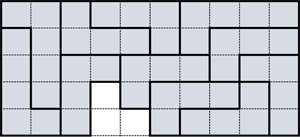
\includegraphics{l-example.jpg}
     \label{obr3}
    \end{center}
    
    \noindent
Mřížka R o rozměrech $10$ x $5$ políček s $3$ zakázanými políčky pokrytá dlaždicemi.

\noindent
Řešení vždy existuje.
\textbf{Těsná dolní mez} na cenu pokrytí je $- 6 \cdot( n \cdot m-k)$, když není vložitelná žádná dlaždice L4/L3.
\textbf{Těsnou horní mez} na cenu pokrytí lze pro dané $m,n,k$ spočítat je možné vypočítat pomocí řešení diofantské rovnice
$4*a+5*b=n*m-k$, které vždy existuje (neboť 4 a 5 jsou nesoudělná čísla) a kde bereme kladné řešení s maximálním $b$. Tuto mez někdy není možné dosáhnout (závisí i na pozici zakázaných políček).


\subsection{Vstupní datové soubory}


Formát vstupního textového datového souboru je následující:

\noindent
1. řádka: celá čísla $m$ a $n$ - rozměry obdélníkové mřížky (počet řádků a sloupců)

\noindent
Další řádka: číslo $k$ - počet zakázaných políček v mřížce
následujících $k$ řádek obsahuje x,y souřadnice zakázaných políček.

\section{Sekvenční řešení}
Sekvenční algoritmus je typu prohledávání do hloubky s metodou větví a hranic (BB-DFS) s hloubkou prohle\-dávaní prostoru omezenou na $(m \cdot n-k)$.
Algoritmus končí, když je cena rovna horní mezi nebo když prohledá celý stavový prostor do hloubky $\frac{m \cdot n-k}{4}
$.

Po načtení dat ze souboru nebo případně z příkazové řádky (obojí lze specifikovat argumenty) jsou vytvořeny dvě instance třídy $sollution$ jedna pro aktuální zpracovávanou konfiguraci a druhá pro nejlepší dozaženou. Mřížku reprezentuju jako 2D vektor a zároveň si držím parametry jako počet prazdných polí za a před zpracovávaným poličkem, počet umístěných kostiček L3 a L4 a také velikost dané mřížky. Celý algoritmus pak využívá pouze dvě metody při řešení. 

První metodou je $nextFree$, která pro zadané souřednice nalezne nejbližší volné políčko (první volání je mimo hrací plochu na začátku). Druhá metoda je pro přídaní políčka na mapu $addOnMap$. Tato metoda bere souřadnici kam začínáme pokládat (pouze pokud lze jinak neproběhne úspěsně), dále relativní souřadnice ve vektoru dané kostičky, předchozí hodnotu na místě a novou hodnotu z counteru. Touto metodou lze také kostičky odebírat pří návratu v DFS při zadání původní hodnoty jako id kostičky, která na místě ležela. 

Z držených parametrů daneho rozložení je vždy spočítána cena a pokud se rovná maximální možné tak algoritmus končí. Dále pro optimalizi používám prořezávání, tedy pokud aktuální instance s teoretickým maximem pro zbývající volná pole nemůže překonat aktuální maximum tak větev také končí.

Níže jsou uvedeny časy sekvenčního řešení pro 3 vybrané instance.
 % jednoduchá tabulka

\begin{center}
\parbox{0cm}{\begin{tabbing}
 město XYZ ~~~~\= datum ~~~~
    \= 34 \kill
    \bfseries Instance \>
    \bfseries Čas (s) \>
    \\[2mm]
    pol13 \> 1091.261 \>  \\
    pol14 \> 640.393 \> \\
    pol15 \> 876.792 \> 
\end{tabbing}}
\end{center}

První instance je prázná pole o rozměrech 22x18. Druhá instance je pole 15x15 s zakazanými políčky v rozích přiblizně prostřed stěn a uprostřed. Poslední je 17x17 se vzorem 4 čverců rozmístěných přibližně symentricky, tak aby kolem sebe měli co nejvíc místa. Tedy celkem 16 zakázaných políček.
\section{Popis paralelního algoritmu a jeho implementace~v~OpenMP~-~taskový paralelismus}
Při implementaci v OpenMP a taskovém paralelismu jsem musel upravil sekvenční řešení. Implementaci pomocí taskového paralelismu ani nebudu dále využívat pro implementaci v MPI. Aby tento paralelismus šlo využít bylo nutné zařídit, aby v rekurzi byla předávána kopie řešení a ne pouze ukazatel na jednu kopii, to celé řešení zpomalovalo a pomocí tohoto řešení se mi nepodařílo dosáhnout obstojných výsledků. 

První použitá direktiva je omp parallel blok a v něm první volání rekurze s direktivou single, je nutné aby první volání provedlo jen jedno vlákno. Samotná rekurze je stejná jako u sekvenčního řešení s těmi rozdíly, že kontrola a update nejlepšího řešení probíhá v kritické sekci a při volaní rekurze a zanoření je použita direktiva omp task, která tvoří tasky. Hloubku zanoření kontroluju podle id kostiček položených na mapě. Tuto hlobku lze nastavit parametrem (-nN) na příkazové řádce stejně jako počet vláken (-nT). Přepínač -tp slouží pro výběr task paralelismu z možností datového (-dp) a nebo pouze rekurzivního na jednom vlákně (-r). Při zkoušení se neosvědčilo mít hloubku zanoření více ja 4 pro 16 jader.

\begin{verbatim}
./[BUILD BINARY] -f [PATH TO INSTANCE] -tp -nT [NUMBER OF THREADS] -nN [PLUNGE DEPTH]
\end{verbatim}


\section{Popis paralelního algoritmu a jeho implementace v OpenMP - datový paralelismus}\label{kap1}

Při implementaci datového paralelismu v OpenMP bylo nutné vytvořit instance problému, které budou distribuované mezi vlákna. Pro toto jsem využil algoritmus BFS, kterým v režimu jednoho vlakna generuje instance (předvyplněné mapy). Počet těchto instancí lze opět určit z příkazové řádky (-nN), ovšem v tomto případě je to minimální počet instancí (dáno větvícím faktorem maximálně o 16 víc), které se vygenerují. 

Pro samotnou implementaci pak využívám direktivu parralel for, který vytvoří daný počet vláken (-nT) a přiděluje jim přegenerované instance. Přidělování používám dynamické. V rekurzi pak pro kontrolu nejlepšího řešení používám direktivu pro kritickou sekci.

Tato implementace paralelního algorimu se mi zamlouvala líp a byla také mnohem efektivnější. To především z důvodu, že jednotlivé vlákna mohou prováděnou rekurzi jednoduše provádět na jedné instanci, což výpočet velice zrychluje. 

\begin{verbatim}
./[BUILD BINARY] -f [PATH TO INSTANCE] -tp -nT [NUMBER OF THREADS] -nN [NUMBER OF GENERATED]
\end{verbatim}


\section{Popis paralelniho algoritmu a jeho implementace v MPI}

Pro MPI bylo nutné přepracovat více části. V MPI je nutné kompilovat kód pomocí speciálního kompilátoru (mpic++) a spouštět pomocí mpirun, kde jsou vytvořeny jednotlivé procesy a je zajištěna komunikace mezi nimi. Implemetace algoritmu je Master-slave. Tedy jeden proces je jako hlavní a ostatní jako dělníci. (v mé pozdější implementaci jsou volná vlákna na masteru také pracující)

Slave proces má jednoduchou implementaci, hlavní částí je blokující příjem zprávy od mastera. V této zprávě bud přijme informaci o konci nebo práci, kterou má vykonávat. Pokud je konec, tak se ukončí. Pokud se jedná o práci, tak vykonává s instancí přesně to, co bylo popsáno v datovém paralelismu v kapitole \ref{kap1}. V kódu je jen jedno vychýlení a to, že po určitěm počtu kroků provádí neblokující broadcastování nejlepšího řešení, tento broadcast začíná vždy master pokud dostane nějaké nové lepší řešení. Toto bylo nezbytně nutné pro ořezavání problému, neboť se stávalo, že zůstával běžet jeden proces (s těžkou úlohou, která mohla být oříznuta), i když řešení bylo dávno nalezeno.

Implementace mastera ze začátku byla pouze na posílání a příjem zpráv. Master má frontu na slave procesy, který má poslat zprávu a neblokujícím send posílá vygenerované instance, která na začátku vygeneroval pomocí BFS stejně jako v datovém paralelismu a kontroluje zda zpráva opravdu odešla. Poté čeká na příchozí zprávu od slave procesu s řešením. Pokud je řešení lepší uloží ho a neblokujícím broadcastem broadcastuje novou nejlepší hodnotu. A Slave procesu pošle novou práci, pokud nějaká je. 

Zprávy v MPI posílám jako pole čísel, kde jsem do objektu řešení vytvořil serializaci právě do pole čísel.

Tuto implemetaci mastera jsem později ještě rozšíříl pomocí OpenMP, kde master umí využít i zbylá vlákna na procesoru k počítání. Používám k tomu zapnuté nested parallel, abych mohl vnořit vytváření vláken pro OpenMP. V masterovi jsou nejprve vytvořena dvě vlákna, kde jedno je klasický master a druhé je jakoby slave. K tomuto řešení jsem pro začátek ještě nastavil zámek, který je zamčený z důvodu, že by se vlákno spustilo dříve, než bude naplněná fronta. Zámek je uvolněn po naplnění fronty. 

Toto slave vlákno pak odebírá problémy z fronty a řeší je datovým paralelismem. Při práci s frontou a nejlepším řešením jsou proměné zamčené v kritické sekci, aby nedocházelo ke konfliktům s master vláknem (procesem). Pří této implementaci se vyskytli nějaké problémy především s kritickými sekcemi, které bylo nutné odladit. Výkonost se ukáže při testování tohoto řešení.

\begin{verbatim}
mpirun -n [NUMBER OF PROCESSES] [BUILD BINARY] -f [PATH TO INSTANCE] -mpi 
-nT [NUMBER OF THREADS] -nN [NUMBER OF GENERATED IN PROCESS] 
-nNP [NUMBER OF GENERATED IN MASTER]
\end{verbatim}

\section{Naměřené výsledky a vyhodnocení}
Zde uvedu naměřené výsledky ze spuštěných experimentů a výpočetním klastru star. Pokusil jsem se neprve zkoumat závislost na velikosti generovaných problémů a to jak na úrovni paralelismu na jednom procesoru, tak na úrovni komunikace mezi vypočetními jednotkami. Dále pak zrychlení s počtem použití výpočetních jader.

\subsection{Závislost výpočetního času na počtu generovaných tasků jeden výpočetní uzel}

Jak je videt na grafech níže je tento problém velice datově závislý a čas velice ovlivní a počet vygenerovaných instancí a to ne v malé míře. Tento test byl prováděn na jednom vypočetním uzlu na 20 jádrech. V tomto případě jsem zde očekával nějakou závislost, ale časy by nejspíš rostly až kdyby generovaní tasků bralo velkou část času, což se děje spíše až uz sta tisíců.


\begin{center}
    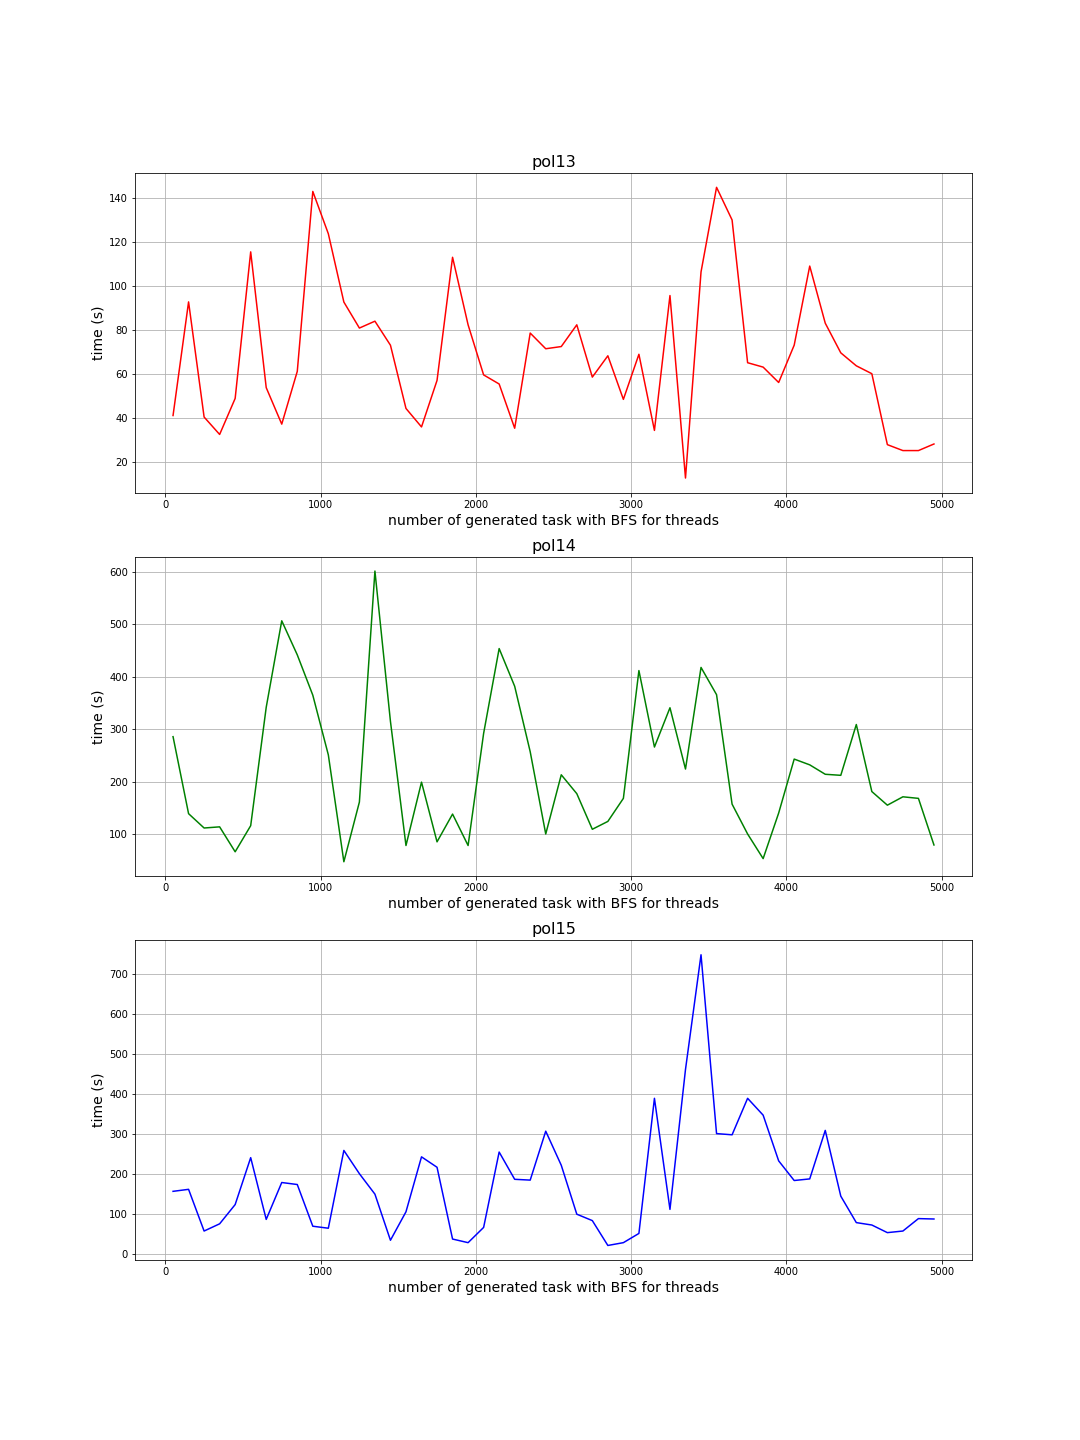
\includegraphics[scale=0.44]{nN.png}
    
     \label{obr1.1}
     
    \end{center}


\subsection{Závislost výpočetního času na počtu generovaných tásků pro MPI}

\subsection{Závislost výpočetního času na počtu vypočetních jader na jednom výpočetním uzlu}

\subsection{Závislost výpočetního času na počtu vypočetních jader v klusteru}

\subsection{Analýza a hodnocení}


Analyza a hodnoceni vlastnosti paralelniho programu, zvlaste jeho efektivnosti a skalovatelnosti, pripadne popis zjisteneho superlinearniho zrychleni.

Škálovatelnost algoritmu je možná v mezích, kdy ještě BFS pro generování tasků bude časově přijatelné k času řešení celého problému. Podle naměřených výsledků bych odhadoval, že lze problém dobře škálovat, protože lze velice rychle vygenerovat velký počet tasků na začátku, ale implemetace algoritmu v MPI by musela být změněna na nějakou, která bude efektivněji využívat síť. V mé implemetaci posílám pokaždé celé zadaní.

\begin{enumerate}
\item Zvolte tri instance problemu s takovou velikosti vstupnich dat, pro ktere ma sekvencni 
algoritmus casovou slozitost kolem 5, 10 a 15 minut.
Pro mereni cas potrebny na cteni dat z disku a ulozeni na disk neuvazujte a zakomentujte
ladici tisky, logy, zpravy a vystupy.
\item Merte paralelni cas pri pouziti $i=2,\cdot,60$ vypocetnich jader na siti Ethernet.
\item Tabulkova a pripadne graficky zpracovan0 namerene hodnoty casove slozitosti měernych instanci behu programu s popisem instanci dat. Z namerenych dat sestavte grafy zrychleni $S(n,p)$. 
\item 

\end{enumerate}

\section{Závěr}

Semestrální práce byla velice zajímavá a práce na ní přínosná především z hlediska ošahání si knihoven pro psaní paralelních programů jinak než přes samotné vytváření vláken pomocí Thread. Tato implementace může být velice efektivní a to především v přehlednosti kódu a časové náročnosti psaní programu. Dále také vyzkoušení si programovaní pro vypočetní klastr, kde je nutné aby spolu jednotlivé procesy komunikovali jinak než přes sdílenou paměť. Semestrální práce nám dala možnost si vyzkoušet různé přístupy a možnost s knihovnami experimentovat.

\end{document}
